\glsresetall{} 
\appendix

\chapter{Algorithms} \label{chap:Algorithms}

%\lettrine[lines=2, findent=0pt, nindent=5pt]{T}{} 

Through the development of the \gls{pops}, a number of algorithms have been
developed to perform various functions. These algorithms are not necessarily
ground breaking but their implementations are novel and worth discussing in
some form. To avoid detracting from the main body of the thesis they are
discussed here, in the appendix.


\section{Multiple Access Intersection Algorithm} \label{alg:mul-access-inter}

For some search scenarios, \gls{pops} may need to determine for what times do all
satellites have access to a target such as an \gls{aoi} or a ground station.
That is, if there are multiple satellites and each satellite has a list of
access times to a target, \gls{pops} must generate a new list of access times where
each access corresponds to a period where all satellites have access. An
example scenario is illustrated in Figure~\ref{fig:access_intersect}.


\begin{figure}[h]
    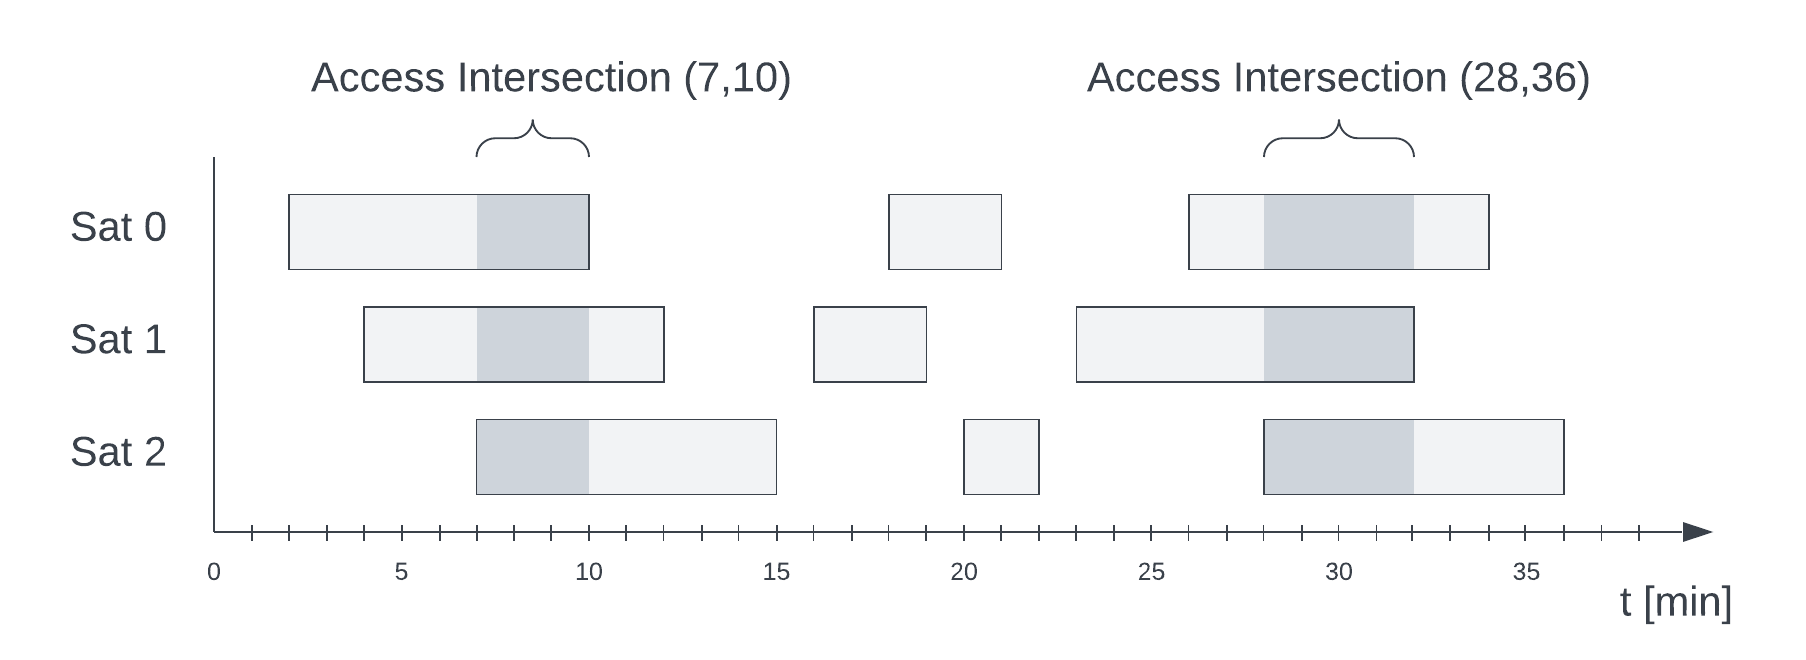
\includegraphics[width=\textwidth]{Access Intersection Example.png} 
    \caption{Illustration of a Potential Access Intersection Scenario}
\label{fig:access_intersect}
\end{figure}

In this scenario, there are three satellites: Sat 0, Sat 1, and Sat 2. Each has
multiple access periods represented with gray boxes. Though time is continuous,
it has been discretized into integer timesteps for simplicity. Minutes have
been selected as the units for time but this is arbitrary. From these lists of
access periods, this algorithm must determine all of the points in time where
all satellites have an access period. For the example scenario, the outputted
results should be $[7,10]$ and $[28,36]$. Note that between $t = 16$ and $t=22$
there are access overlaps but since there are only overlaps between two
satellites, they should not be returned as intersection periods.

For each satellite, access times are stored as a list of timestamps. Every even
and odd indexed timestamp specifies when the satellite `enters' and `leaves' an
access respectively. Access lists $\ses{a}{n}$ can be described generally for
satellite $n$ as,

\begin{equation}\label{eq:access-list} 
    \ses{a}{n} = \left[ a_{n,0}, b_{n,0}, a_{n,1}, b_{n,1}, \ldots a_{n,m}, b_{n,m} \right]
\end{equation}


where $a$ is the access enter timestamp, $b$ is the access leave timestamp, and
$m$ is the number of accesses. We also make the assumption that no accesses
overlap for a given satellite and target; that is,

\begin{equation}\label{eq:access-list-constraint}
    a_{n,0} < b_{n,0} < a_{n,1} < b_{n,1} < \ldots < a_{n,m} < b_{n,m}
\end{equation}

One simple brute force solution to this problem would be to iterate over every
time step, $t$, and check if there exists an access region, $[a_n,b_n]$, for all
satellites, $n$, such that $t$ is between $a$ and $b$.

This solution is, of course, very wasteful as it scales with the number of
timesteps that are being considered, $\Theta(t)$. The number of timesteps may
be on the order of 1,000s to 10,000s of timesteps. A simplification can be made
since we do not need to actually consider every timestep. Rather, we can
instead iterate over the access boundaries since they describe continuous
periods of time. By focusing on just the access boundaries, we may develop an
algorithm which scales with the number of accesses, $\Theta(m)$, which is much
smaller than the total number of timesteps.

For all satellite access lists we are considering, let us combine them into two
$1\times nm$ arrays. The first `timestamp' array, $\se{b}$, contains a sorted
list of all of the boundary timestamps in ascending order. The second `index'
array, $\se{s}$, contains a list of satellite indices in the same order as the
timestamp array. For example,

\begin{equation*}
    \begin{aligned} 
	\ses{a}{0} &= \left[ 2, 10, 18, 21  \right] \\
	\ses{a}{1} &= \left[ 4, 12, 16, 19  \right] \\
	\ses{a}{2} &= \left[ 7, 15, 20, 22  \right] \\
    \end{aligned}
    \quad \Rightarrow \quad
    \left \{ 
	\begin{aligned}
	    \se{b} &= [ 2 , 4 , 7 , 10 , 12 , 15 , 16 , 18 , 19 , 20 , 21 , 22  ] \\
	    \se{s} &= [ 0 , 1 , 2 , 0 , 1 , 2 , 1 , 0 , 1 , 2 , 0 , 2  ]
	\end{aligned}
    \right.
\end{equation*}

Note these are some of the values from Figure \ref{fig:access_intersect}.
Again, in the actual implementation of the algorithm we use actual timestamps
but here we are using integers for demonstration purposes. The timestamp array
stores the timestamp of the access boundary for later reference and also gives
us the order of the satellite index array. Remember that access boundaries are
listed in order of [enter, leave, enter, leave, ...]. Looking at the first four
elements in the index array, $[0, 1, 2, 0]$, satellite 0 enters an access at
the first element and leaves the access at the fourth element. So for the
second and third element, satellite 0 still has access because it has not left
yet. In essence, the index array encodes in what order satellites enter and
leave accesses. 

Now let us expand on the index array so we can perform logical operations to
find intersections. For this the algorithm makes use of logic arrays.  These
are arrays which contain only Boolean values, True or False. With these arrays,
we can also perform logical operations on any axis. For example, if we have a 2
dimensional logic array, we can produce a 1 dimensional array, that is the
result of AND'ing all of the elements in each column. These allow us to perform
logical operations very quickly for many elements. From the index array let us
construct an $n\times nm$ boolean array, $\se{A}$, that describes our scenario.
The rows of matrix, $\se{A}$, correspond to the indices of each satellite.  For
example row 0 is satellite 0, row $m$ is satellite $m$, etc. The columns
correspond to elements in the index array, $\se{s}$.

Let us initialize $\se{A}$ to be all False values represented as 0s. Then,
starting at the first column of $\se{A}$, let us NOT the element in the
$\se{s}(0)$ row.  Then, for then next column, let us copy all of the values
from the previous column and again NOT the $\se{s}(1)$ element. This is then
repeated for all columns in $\se{A}$. There is one small catch, if we are
transitioning a 1 to a 0 or a True to a False, this should be done on the
following iteration. This essentially means that we are treating accesses in
access boundaries as inclusive. Even if the satellite is leaving an access, we
say that it has access until the timestep immediately after the boundary. As an
example, let us construct $\se{A}$ from $\se{s}$ for all of Figure
\ref{fig:access_intersect},

\begin{equation*} 
    \se{s} = 
    \left[
    \begin{array}{cccccccccccccccccc}
	0 & 1 & 2 & 0 & 1 & 2 & 1 & 0 & 1 & 2 & 0 & 2 & 1 & 0 & 2 & 1 & 0 & 2 \\
    \end{array}
    \right]
\end{equation*}
yields,
\begin{equation*} 
    \se{A} = 
    \left[
	\begin{array}{cc;{2pt/2pt}cc;{2pt/2pt}cccccccccc;{2pt/2pt}cc;{2pt/2pt}cc}
	1 & 1 & 1 & 1 & 0 & 0 & 0 & 1 & 1 & 1 & 1 & 0 & 0 & 1 & 1 & 1 & 1 & 0 \\
	0 & 1 & 1 & 1 & 1 & 0 & 1 & 1 & 1 & 0 & 0 & 0 & 1 & 1 & 1 & 1 & 0 & 0 \\
	0 & 0 & 1 & 1 & 1 & 1 & 0 & 0 & 0 & 1 & 1 & 1 & 0 & 0 & 1 & 1 & 1 & 1 \\
    \end{array}
    \right]
\end{equation*}
Then, if we AND all of the rows in $\se{A}$ we get,
\begin{equation*} 
    \se{A}' = 
    \left[
    \begin{array}{cccccccccccccccccc}
	0 & 0 & 1 & 1 & 0 & 0 & 0 & 0 & 0 & 0 & 0 & 0 & 0 & 0 & 1 & 1 & 0 & 0 \\
    \end{array}
    \right]
\end{equation*}
It is clear to see that this matrix gives us the indices where there is an
intersection between all satellites. If we take all values of $\se{b}$ where
$\se{A}'$ is True, we are left with,
\begin{equation*} 
    \se{b}' = 
    \left[
    \begin{array}{cccccccccccccccccc}
	7 & 10 & 28 & 32
    \end{array}
    \right]
\end{equation*}
which is our expected result. This was just a walkthrough but the explicit
algorithm definition is defined in Algorithm~\ref{alg:access-intersection}.

\begin{algorithm}[h] 
    \caption{Access Intersection} 
    \label{alg:access-intersection}
    \begin{algorithmic}[1]
	%\Require{\se{z}is a $1\times N$ array } 
	\Function{AccessIntersection}{$\ses{a}{0}$,$\ses{a}{1}$, ... , $\ses{a}{n}$} 

	    \Let{$\se{s}$, $\se{b}$}{\Call{Combine}{$\ses{a}{0}$,$\ses{a}{1}$, ... , $\ses{a}{n}$}}  

	    \Let{$l$}{\Call{Length}{$\se{s}$}}

	    \Let{$\se{A}$}{\Call{Zeros}{$n$,$l$}}

	    %\Let{$\se{A}[\se{s}[0],0]$}{1}  \Comment{Set up the first column}
	    \Let{$\se{t}$}{$\se{A}[:,0]$} \Comment{Temporary array to store column of $\se{A}$}

	    \Let{$i$}{0} \Comment{Boundary iterator}

	    \While{$i \neq m$}
		\Let{$s$}{$\se{s}[i]$} \Comment{Satellite index}
		
		\If{!$\se{t}$($s$)}
		\Let{$\se{t}$($s$)}{!$\se{t}$($s$)}
		    \Comment{Flip element then copy values over}
		    \Let{$\se{A}[:,s]$}{\Call{OR}{$\se{A}[:,s]$, $\se{t}$}} 
		\Else
		    \Let{$\se{A}[:,s]$}{\Call{OR}{$\se{A}[:,s]$, $\se{t}$}} 
		    \Comment{Copy values over then flip element}
		    \Let{$\se{t}$($s$)}{!$\se{t}$($s$)}
		\EndIf


		\Let{$i$}{$i+1$}
	    \EndWhile 

	    \Let{$\se{a}'$}{\Call{ColumnsAND}{$\se{A}$}}

	    \Let{$\se{b}'$}{$\se{b}[\se{a}']$} \Comment{Select indices based on logical value}

	\State \Return $\se{b}'$
	\EndFunction
    \end{algorithmic}


\end{algorithm}

For this algorithm, the implementation of \textsc{Combine} function was omitted
for clarity since it is an implementation detail. Also, note that this
algorithm is not limited to only access intersections but it may also calculate
unions by replacing \textsc{ColumnsAND} with \textsc{ColumnsOR} in line 18.

%%%%%%%%%%%%%%%%%%%%%%%%%%%%%%%%%%%%%%%%%%%%%%%%%%%%%%%%%%%%%%%%%%%%%%%%%%%%%% 

%\section{Equator Crossing Algorithm} \label{sec:equator-crossing}
%
%For a given ephemeris, it is useful to determine each `pass' of that orbit.
%That is, for each ephemeris point, an index should be assigned to it which
%indicates how many times the spacecraft has orbited the Earth. In this way, if
%we have some time range and we wish to see the next `pass,' we would simply
%take that time range's pass index and add 1.
%
%There are many ways a pass may be defined. For example, we could specify a
%latitude and longitude range and whenever the spacecraft is in this range, that
%could be considered a singular pass.  Generally, though, ephemeris data is not
%given in latitude or longitude, rather it is given in a Cartesian position in
%some \gls{eci} or \gls{ecef} coordinate reference frame. So, for each position
%in the ephemeris, the position vector will need to be converted to latitude and
%longitude. 
%
%This is a completely acceptable approach but we may also simplify the problem.
%Instead of taking a latitude and longitude range, we could instead increment
%the pass index when the spacecraft crosses the equator and goes from the
%southern to the northern hemisphere. This would be when the spacecraft's
%position goes from a negative to a positive latitude. This definition of a pass
%has a few advantages. That being, we only need to do one check to determine a
%pass boundary. It also has the benefit of indexing the entire ephemeris. Still
%for this method, we need to convert from Cartesian position to at least
%latitude.
%
%Let us make one further simplification by assuming that the x-y plane of the
%ephemeris's coordinate system is very near to the Earth's equatorial plane.
%This is not true for all coordinate systems but it is true for the \gls{ecef}
%ephemerides used by \gls{pops}. By making this assumption, we no longer need to
%calculate the latitude of the spacecraft; rather, we can instead only look at
%the spacecraft's position along the z-axis. This is useful because the
%spacecraft's z-position will oscillate between some positive and negative
%extrema, which are determined by the orbit's inclination and eccentricity. 
%
%There is a complicating factor that should be accounted for. In time, the
%spacecraft's position is periodic, but when considering only the spacecraft's
%z-position in an ephemeris, there is no guarantee that there is a constant
%timestep between position values. Additional data-points may be injected for
%periods where greater accuracy is desired and vice-versa. 
%
%We may now articulate the problem to be addressed: Given, an array of
%$z$-positions, $\se{z}$, generate a new array, $\se{p}$, that each element of
%$\se{p}$ is the index of an element in $\se{z}$ after a crossover occurs (i.e.\
%the positive value in the negative-to-positive crossing). To determine if
%elements, $n$ and $m$, of an array, $\se{z}$, form a crossover, they must
%satisfy three simple conditions:
%
%\begin{enumerate}
%    \item $\se{z}[n] < 0$
%    \item $\se{z}[m] > 0$ 
%    \item $m = n+1$
%\end{enumerate}
%
%
%A brute-force approach to finding $\se{p}$ would be to loop through all of the
%elements in $\se{z}$ and test them against the above conditions. This method,
%though, is inelegant and may be computationally intensive.  
%
%Alternatively, we can instead try and make use of 
%
%Another approach to
%this problem is outlined in Algorithm~\ref{alg:crossover}.  In essence, it
%attempts to reduce the number of comparisons made to search for crossovers. 
%
%\begin{algorithm}[h] 
%    \caption{Negative-Positive Crossing Search Algorithm} 
%    \label{alg:crossover}
%    \begin{algorithmic}[1] 
%	\Require{\se{z}is a $1\times N$ array } 
%
%	\Function{FindAllCrossovers}{$s, f, \se{z}$}
%	    \Let{$p$}{\Call{FindNextCrossover}{$0, s, f, \se{z}$}} \Comment{Start at beginning of array}
%	    \Let{$\se{p}$}{$\{ p \}$}
%
%	    \While{$p \neq -1$}
%		\Let{$p$}{\Call{FindNextCrossover}{$p, s, f, \se{z}$}}
%		\Comment{Start at beginning of array} \State
%		$\se{p}$.append($p$) \EndWhile 
%		\State \Return \se{p}
%	\EndFunction
%
%	\State
%
%	\Function{FindNextCrossover}{$i, s, f, \se{z}$} 
%	\Let{$j$}{$i+s$}
%	\If{$j > length(\se{z})$} 
%	    \State $s = \mathrm{s \times f}$  
%	\ElsIf{$j = length(\se{z})$}
%	    \State \Return $-1$	  \Comment{Search has completed}
%	\ElsIf{ $(\se{z}[i] < 0) \lor (\se{z}[j] > 0)$ }
%	    \If{$s=1$}
%	    \State \Return $i$ \Comment{Crossover index found}
%	    \Else
%		\State $s = ceil(s \times f)$
%	    \EndIf
%	\Else
%	    \State $i=j$
%	\EndIf
%	\State \Return \Call{FindNextCrossover}{$i, s, f, \se{z}$}
%	\EndFunction 
%    \end{algorithmic} 
%\end{algorithm}


%%%%%%%%%%%%%%%%%%%%%%%%%%%%%%%%%%%%%%%%%%%%%%%%%%%%%%%%%%%%%%%%%%%%%%%%%%%%%% 

\section{Single Access Intersection Algorithm} \label{alg:contains}

The Single Access Intersection Algorithm is similar to the Multiple Access
Intersection algorithm but it serves a different purpose. Given a time range,
this algorithm is concerned with finding all of the access times in a list that
intersect that time range. Here, the input time range will not be used as
bounds, but only search criteria to select access times. 

\begin{figure}[h]
    \centering
    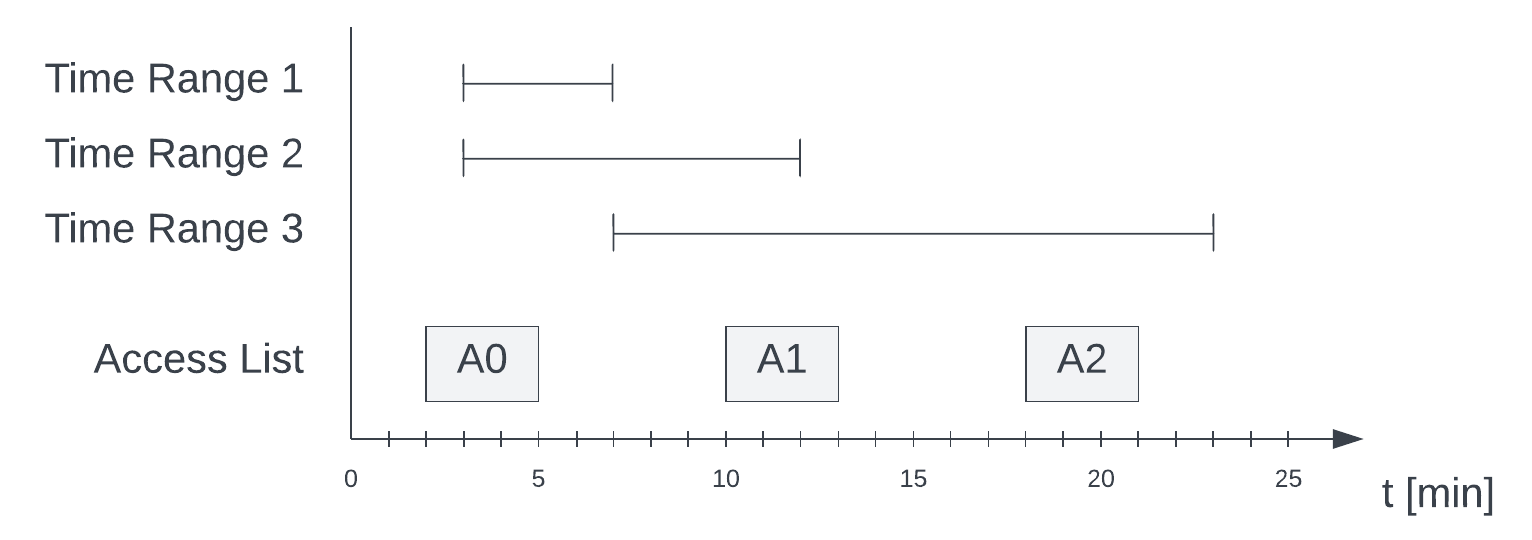
\includegraphics[width=\textwidth]{Single Access.png} 
    \caption{Illustration of a Potential Single Intersection Scenarios}
    \label{fig:single-access-intersect}
\end{figure}

To get a better idea of the problem, let us look at some more concrete example
scenarios. Figure~\ref{fig:single-access-intersect} illustrates an access list
as well as three possible input time ranges, Time Range 1-3. For Time Range 1,
the output should be merely A0. For Time Range 2, the output will be A0 and A1.
Lastly, Time Range 3 will have outputs A1 and A2. Notice here that the limits
of the time range may lie within or without an access. As long as the access
intersects the time range at all, it should be included.

The two inputs to this algorithm are a time region with boundaries $\alpha$ and
$\beta$ where $\alpha < \beta$. The access list, $\se{a}$, is the same as
described in (\ref{eq:access-list}) where the subscript, $n$ has been omitted
since only one access list is to be considered. Additionally, the assumption in
(\ref{eq:access-list-constraint}) still holds here. It should be emphasized
that given an access list, every even entry is an access enter timestamp and
every odd entry is an access leave timestamp.

The main intuition for this problem is that we must first constrain the list of
access boundaries to the those boundaries that lie within the time range.
Then, we must assemble the access times from their boundaries and output them
in a list.  

First we find two values, $i$ and $j$.  These are the indices of the next
smallest value for $\alpha$ and $\beta$ in the access list.  For example, in
Time Range 2, from Figure~\ref{fig:single-access-intersect}, $i$ and $j$ will
be the indices of $a_0$ and $a_1$ respectively. These two values will be used
to create an iteration range that will be used to return the list of accesses. 

One problem is that, as they are, $i$ may not point to an access enter and $j$
may not point to an access leave which is required by access lists. So, if $i$
points to an access enter, nothing should be done but if it points to an access
leave, it should be incremented to point to the next access enter. Similarly,
if $j$ points to an access leave nothing should be done, but if it points to an
access enter it should be incremented as well.  To address this, we may take
advantage of the access list's even and oddness as mentioned earlier.  With
modular arithmetic, we can select the correct indices,

\begin{align*}
    i' &= i + \mathrm{mod}(i,2) \\
    j' &= j + \mathrm{mod}(j+1,2)
\end{align*}
where $i'$ and $j'$ are the shifted indices and `mod()' is the modulus
function.  The first argument is the dividend and the second is the divisor.
Once we have these values, the output will be the access times that lie within
the range $[i', j']$. All together, the algorithm can be seen in
Algorithm~\ref{alg:single-access-intersection}.


\begin{algorithm}[h] 
    \caption{Single Access Intersection}
    \label{alg:single-access-intersection} 
    \begin{algorithmic}[1]
	%\Require{\se{z}is a $1\times N$ array } 
	\Function{SingleAccessIntersection}{$\alpha$, $\beta$, $\se{a}$} 

	\Let{$i$}{$\se{a}[-1]$}
	\Let{$j$}{$\se{a}[-1]$} \Comment{Initialize}

	\ForEach{$t$ in $\se{a}$} \Comment{Find next smallest }
	    \If{ $t < \alpha$ }
	    \Let{$i$}{$t$}  
	    \EndIf
	    \If{ $t < \beta$ }
		\Let{$j$}{$t$}
	    \EndIf
	\EndFor

	\Let{$i'$}{$i + \mathrm{mod}(i,2)$} \Comment{Increment indices}
	\Let{$j'$}{$i + \mathrm{mod}(j+1,2)$} 

	\If{$i > j$}
	    \State \Return $[]$ \Comment{No Access Found}
	\Else
	    \State \Return $\se{a}[i',j']$ \Comment{Return list of access times}
	\EndIf
	\EndFunction
    \end{algorithmic}
\end{algorithm}

This algorithm is very simple and straightforward but it still serves a useful
function. Determining if ground station accesses lie between two accesses may
be calculated hundreds of times in a single search, so it is important that
this calculation is quick and efficient.


%%%%%%%%%%%%%%%%%%%%%%%%%%%%%%%%%%%%%%%%%%%%%%%%%%%%%%%%%%%%%%%%%%%%%%%%%%%%%% 

\section{Swath Boundary Ellipse Algorithm} \label{alg:ellipse}

To review, Swaths are the area covered by a satellite's \gls{fov} footprint or
\gls{for} access region over time. They are calculated from a satellite
ephemeris, where for each telemetry point in the ephemeris, two swath boundary
points are generated. By combining these points together over an entire
ephemeris, we are given two polylines which form the boundaries of the swath,
$L_1$ and $L_2$. If we look in the same direction and the velocity vector of
the satellite at a single time instant, $L_1$ is to the left and $L_2$ is to
the right. Though this is not always the case, the \gls{fov} or \gls{for} of
satellites in \gls{pops} are assumed to be conical. As such, for each ephemeris
point the swath is calculated from, an elliptical footprint/access region is
approximated through a list of some number of points. For clarity, these points
grouped together are referred to as an `Ellipse', $E$, just so that we do not
need to distinguish between footprints and access regions.  

Suppose we wish to more accurately display a swath by including the ellipse
points at the boundaries. Our main problem is that we must determine what
points in the first, $E_{start}$, and last, $E_{end}$ ellipse lie `outside' of the
swath.  If they are inside the swath, they provide no new information and do
not lie on the boundary.  We must also omit points on the ellipses that can be
found on the boundary lines since they are already accounted for. Also, for
robustness, let us assume that the list of points in each Ellipse are not
necessarily in order. This may be the case but this saves us from having to
rely on convention which may be broken in the future.

\begin{figure}[h]
    \centering
    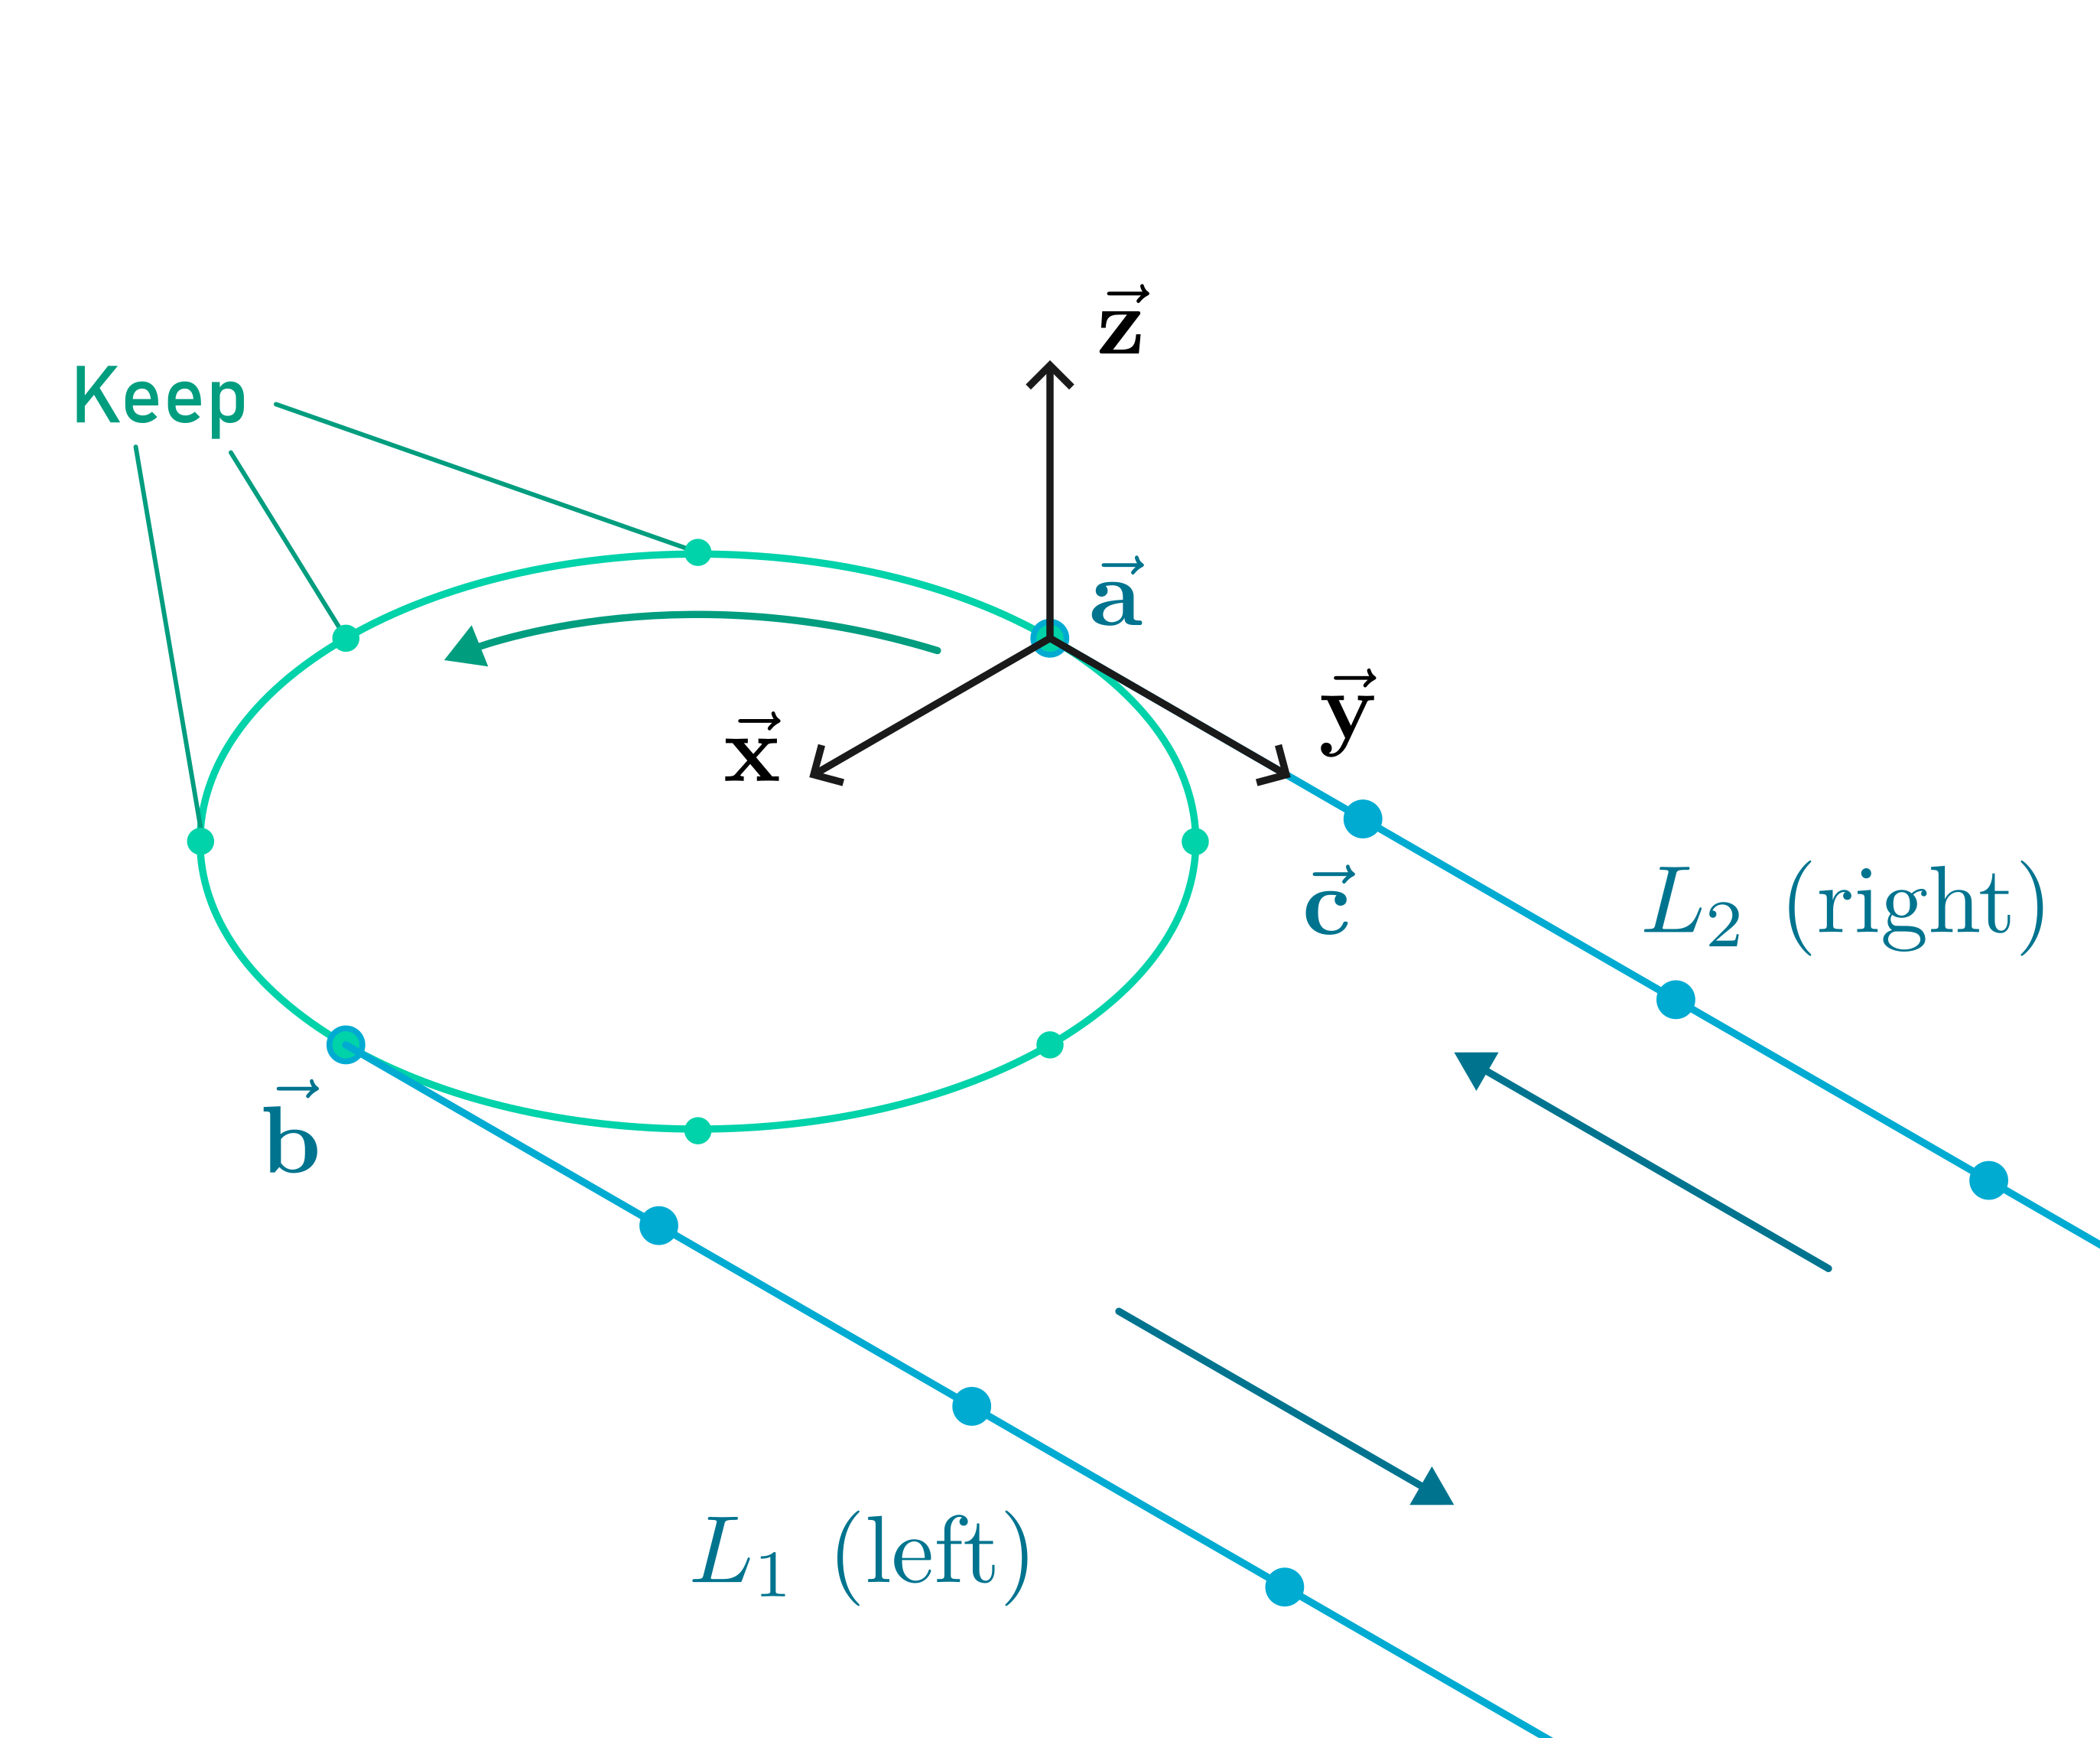
\includegraphics[width=0.7\textwidth]{Swath-Edge.png} 
    \caption{Swath Edge Illustration}
    \label{fig:swath-edge}
\end{figure}

%\newcommand{\a}{$\sesv{a}$} 

\newcommand{\Fs}{$\vec{\mathcal{F}}_s$} 
%\newcommand{\Fe}{$\vec{\mathcal{F}}_E$}

This is the procedure for finding the `outside' points on one end of a swath as
illustrated in Figure~\ref{fig:swath-edge}. First, we take the positions of the
two last points of the boundary lines, $\sev{a}$ and $\sev{b}$, defined in
\gls{ecef} coordinates, \Fe. If we look down the length of a swath towards the
end we are calculating ellipse points for, point $a$ is on the right and point
$b$ is on the left.  Let us also take the position of a third point, $\sev{c}$,
which is the second last point on the right boundary line.  From these points,
we can define a coordinate reference frame, \Fs $= [\seh{x}, \seh{y},
\seh{z}]$, with respect to \Fe, where:

\begin{equation}
    \seh{x} = \frac{\sev{b}-\sev{a}}{\norm{\sev{b} - \sev{a}}}
    , \quad
    \seh{y} = \frac{\sev{c}-\sev{a}}{\norm{\sev{c} - \sev{a}}}
    , \quad
    \seh{z} = \seh{x} \times \seh{y}
\end{equation}

In this reference frame, all of the ellipse points that are outside the swath
will have negative y-components. To determine this, we can project each point
in the ellipse onto the x-y plane of \Fs~and then take the dot product of the
projected point with $\seh{y}$. To order the edge points such that they
correctly form the boundary, we can take the dot product of the projected point
and $\seh{x}$ and then store them in ascending order. This procedure yields
the algorithm in Algorithm~\ref{alg:swath-edge}.

%% NOTE: this is not how it's defined in the code. Here it's been reversed for clarity

\begin{algorithm}
    \caption{Swath Edge Algorithm} 
    \label{alg:swath-edge}
    \begin{algorithmic}[1] 
	\Function{SwathEdge}{$L_1, L_2, E$}
	\Let{$\sev{a}$}{$L_2[-1]$}	\Comment{Last Point}
	\Let{$\sev{b}$}{$L_1[0]$}	\Comment{First Point}
	\Let{$\sev{c}$}{$L_2[-2]$}	\Comment{Second Last Point}
	\Let{$\seh{x}$}{$\sev{b}-\sev{a}/\norm{\sev{b}-\sev{a}}$}
	\Let{$\seh{y}$}{$\sev{c}-\sev{a}/\norm{\sev{c}-\sev{a}}$}
	\Let{$\seh{z}$}{$\seh{x} \times \seh{y}$}

	\ForEach{Ellipse Point $\sev{e}$ in $E$}
	    \Let{$\sesv{p}{e}$}{$\sev{e} - (\sev{e}\cdot\seh{z})\seh{z}$} 
	    \Comment{Projection onto x-z plane}

	    \If {$(\sesv{p}{e} \cdot \seh{y}) < 0 $}
		\Let{$O$}{\Call{InsertSorted}{$\sev{e}$, $(\sesv{p}{e}\cdot\seh{x})$, $O$}}
		\Comment{Sort in Descending order}
	    \EndIf
	\EndFor
	\State \Return $O$
	\EndFunction
    \end{algorithmic} 
\end{algorithm}

When providing points to this algorithm, it is assumed that the points in $L_1$
and $L_2$ are ordered Counter Clockwise. Also, sorting algorithms are not the
focus here so the implementation of \textsc{InsertSorted} has been omitted for
clarity.  This was the procedure for finding the swath edge for the start of
the swath.  To find the edge for the end, we can use the same algorithm but
switch $L_1$ and $L_2$, and pass the Ellipse at the end of the swath. In so
doing, we have flipped $L_1$ to be the right side of the swath instead of the
left and vice-versa for $L_2$. 

%%%%%%%%%%%%%%%%%%%%%%%%%%%%%%%%%%%%%%%%%%%%%%%%%%%%%%%%%%%%%%%%%%%%%%%%%%%%%% 

%\section{Counter-Clockwise Reordering Algorithm} \label{alg:ccw}

%%%%%%%%%%%%%%%%%%%%%%%%%%%%%%%%%%%%%%%%%%%%%%%%%%%%%%%%%%%%%%%%%%%%%%%%%%%%%% 

%\section{Convex Polygon Conversion} \label{alg:force-complex}

